% Options for packages loaded elsewhere
\PassOptionsToPackage{unicode}{hyperref}
\PassOptionsToPackage{hyphens}{url}
%
\documentclass[
  letterpaper,
  ignorenonframetext,
  aspectratio=43,
  handout,
  12pt]{beamer}
\usepackage{pgfpages}
\setbeamertemplate{caption}[numbered]
\setbeamertemplate{caption label separator}{: }
\setbeamercolor{caption name}{fg=normal text.fg}
\beamertemplatenavigationsymbolsempty
% Prevent slide breaks in the middle of a paragraph
\widowpenalties 1 10000
\raggedbottom
\setbeamertemplate{part page}{
  \centering
  \begin{beamercolorbox}[sep=16pt,center]{part title}
    \usebeamerfont{part title}\insertpart\par
  \end{beamercolorbox}
}
\setbeamertemplate{section page}{
  \centering
  \begin{beamercolorbox}[sep=12pt,center]{part title}
    \usebeamerfont{section title}\insertsection\par
  \end{beamercolorbox}
}
\setbeamertemplate{subsection page}{
  \centering
  \begin{beamercolorbox}[sep=8pt,center]{part title}
    \usebeamerfont{subsection title}\insertsubsection\par
  \end{beamercolorbox}
}
\AtBeginPart{
  \frame{\partpage}
}
\AtBeginSection{
  \ifbibliography
  \else
    \frame{\sectionpage}
  \fi
}
\AtBeginSubsection{
  \frame{\subsectionpage}
}
\usepackage{lmodern}
\usepackage{amssymb,amsmath}
\usepackage{ifxetex,ifluatex}
\ifnum 0\ifxetex 1\fi\ifluatex 1\fi=0 % if pdftex
  \usepackage[T1]{fontenc}
  \usepackage[utf8]{inputenc}
  \usepackage{textcomp} % provide euro and other symbols
\else % if luatex or xetex
  \usepackage{unicode-math}
  \defaultfontfeatures{Scale=MatchLowercase}
  \defaultfontfeatures[\rmfamily]{Ligatures=TeX,Scale=1}
\fi
\usetheme[]{metropolis}
% Use upquote if available, for straight quotes in verbatim environments
\IfFileExists{upquote.sty}{\usepackage{upquote}}{}
\IfFileExists{microtype.sty}{% use microtype if available
  \usepackage[]{microtype}
  \UseMicrotypeSet[protrusion]{basicmath} % disable protrusion for tt fonts
}{}
\makeatletter
\@ifundefined{KOMAClassName}{% if non-KOMA class
  \IfFileExists{parskip.sty}{%
    \usepackage{parskip}
  }{% else
    \setlength{\parindent}{0pt}
    \setlength{\parskip}{6pt plus 2pt minus 1pt}}
}{% if KOMA class
  \KOMAoptions{parskip=half}}
\makeatother
\usepackage{xcolor}
\IfFileExists{xurl.sty}{\usepackage{xurl}}{} % add URL line breaks if available
\IfFileExists{bookmark.sty}{\usepackage{bookmark}}{\usepackage{hyperref}}
\hypersetup{
  hidelinks,
  pdfcreator={LaTeX via pandoc}}
\urlstyle{same} % disable monospaced font for URLs
\newif\ifbibliography
\usepackage{graphicx}
\makeatletter
\def\maxwidth{\ifdim\Gin@nat@width>\linewidth\linewidth\else\Gin@nat@width\fi}
\def\maxheight{\ifdim\Gin@nat@height>\textheight\textheight\else\Gin@nat@height\fi}
\makeatother
% Scale images if necessary, so that they will not overflow the page
% margins by default, and it is still possible to overwrite the defaults
% using explicit options in \includegraphics[width, height, ...]{}
\setkeys{Gin}{width=\maxwidth,height=\maxheight,keepaspectratio}
% Set default figure placement to htbp
\makeatletter
\def\fps@figure{htbp}
\makeatother
\setlength{\emergencystretch}{3em} % prevent overfull lines
\providecommand{\tightlist}{%
  \setlength{\itemsep}{0pt}\setlength{\parskip}{0pt}}
\setcounter{secnumdepth}{-\maxdimen} % remove section numbering
\usepackage{pgfpages}
\pgfpagesuselayout{2 on 1}
\providecommand{\tightlist}{%
\setlength{\itemsep}{0pt}\setlength{\parskip}{0pt}}
\makeatletter
\makeatother
\let\Oldincludegraphics\includegraphics
\renewcommand{\includegraphics}[2][]{\Oldincludegraphics[width=\textwidth,height=0.7\textheight,keepaspectratio]{#2}}
\ifluatex
  \usepackage{selnolig}  % disable illegal ligatures
\fi

\author{}
\date{}

\begin{document}

\begin{frame}{Mechanics of Materials}
\protect\hypertarget{mechanics-of-materials}{}
Lecture 15 - Combined Loading

Dr.~Nicholas Smith

Wichita State University, Department of Aerospace Engineering

13 October, 2020
\end{frame}

\begin{frame}{schedule}
\protect\hypertarget{schedule}{}
\begin{itemize}
\tightlist
\item
  13 Oct - Combined Loading, HW 6 Self-Grade Due
\item
  15 Oct - Stress Transformation
\item
  20 Oct - Stress Transformation, HW 7 Due
\item
  22 Oct - Strain Transformation
\end{itemize}
\end{frame}

\begin{frame}{outline}
\protect\hypertarget{outline}{}
\begin{itemize}
\tightlist
\item
  pressure vessels
\item
  combined loading
\item
  group problems
\end{itemize}
\end{frame}

\begin{frame}{thin-walled pressure vessels}
\protect\hypertarget{thin-walled-pressure-vessels}{}
\begin{itemize}
\tightlist
\item
  If the radius to wall thickness ratio is 10 or more, we can treat a
  pressure vessel as ``thin-walled''
\item
  Cylindrical pressure vessels will have two primary sources of stress,
  and serve as an introduction to more general states of combined
  loading
\end{itemize}
\end{frame}

\begin{frame}{cylindrical vessels}
\protect\hypertarget{cylindrical-vessels}{}
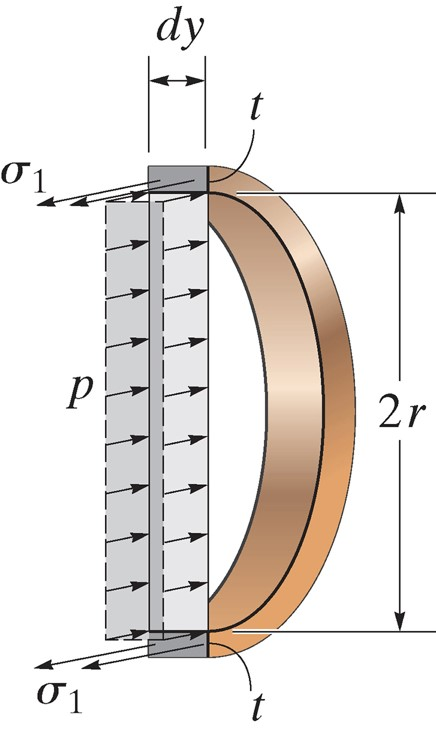
\includegraphics{../images/cylinder-slice.jpg}
\end{frame}

\begin{frame}{cylindrical vessels}
\protect\hypertarget{cylindrical-vessels-1}{}
\begin{itemize}
\tightlist
\item
  From equilibrium of a section of a cylindrical vessel, we see that
\end{itemize}

\[\begin{aligned}
  \sum F_x &= 0\\
  &= 2(\sigma_1 t dy) - p (2r) dy\\
  \sigma_1 &= \frac{pr}{t}
\end{aligned}\]
\end{frame}

\begin{frame}{cylindrical vessels}
\protect\hypertarget{cylindrical-vessels-2}{}
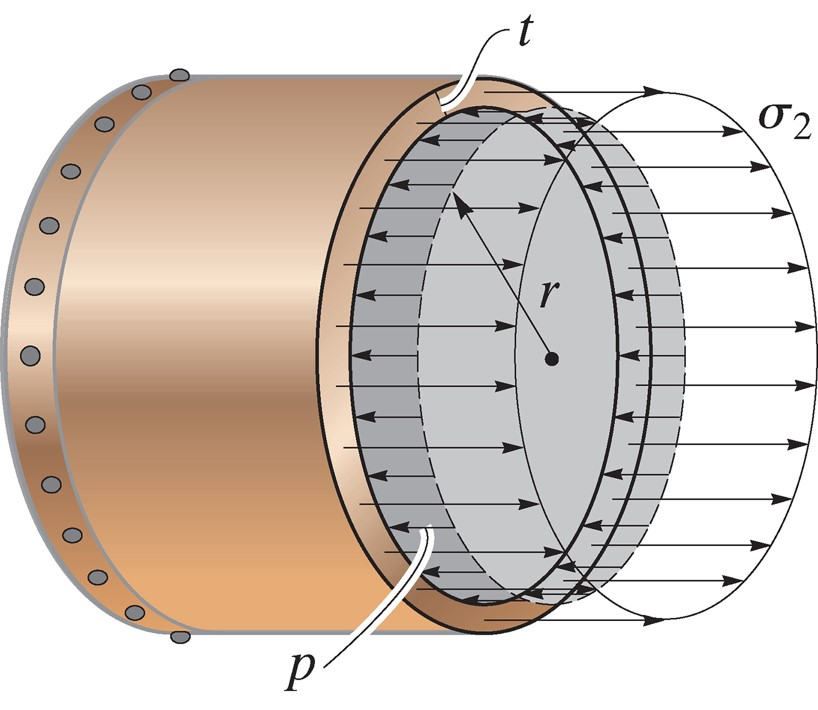
\includegraphics{../images/cylinder-end.jpg}
\end{frame}

\begin{frame}{cylindrical vessels}
\protect\hypertarget{cylindrical-vessels-3}{}
\begin{itemize}
\tightlist
\item
  Considering another section we can find the longitudinal stress
\end{itemize}

\[\begin{aligned}
  \sum F_y &= 0\\
  &= \sigma_2 (2\pi rt) - p (\pi r^2)\\
  \sigma_2 &= \frac{pr}{2t}
\end{aligned}\]
\end{frame}

\begin{frame}{spherical vessels}
\protect\hypertarget{spherical-vessels}{}
\begin{itemize}
\tightlist
\item
  We can find the stress in spherical vessels using an identical section
  to the longitudinal section for a cylindrical vessel, and we find that
\end{itemize}

\[\sigma = \frac{pr}{2t}\]

\begin{itemize}
\tightlist
\item
  Which is valid everywhere in a cylindrical vessel
\end{itemize}
\end{frame}

\begin{frame}{example 8.1}
\protect\hypertarget{example-8.1}{}
\begin{itemize}
\tightlist
\item
  A cylindrical pressure vessel has an inner diameter of 4 ft and a
  thickness of 1/2 in.
\item
  Determine the maximum internal pressure it can sustain if the maximum
  stress it can support is 20 ksi.
\item
  What is the maximum internal pressure a spherical pressure vessel
  could sustain under identical conditions?
\end{itemize}
\end{frame}

\begin{frame}{combined loading}
\protect\hypertarget{combined-loading}{}
\begin{itemize}
\tightlist
\item
  We can use the principle of superposition to treat various loading
  conditions separately and then add them together to find the total
  stress
\end{itemize}
\end{frame}

\begin{frame}{procedure}
\protect\hypertarget{procedure}{}
\begin{itemize}
\tightlist
\item
  Section the member at the point of interest, internal force components
  should be drawn acting through the centroid of the section
\item
  Moment components should be calculated about the centroidal axis
\end{itemize}
\end{frame}

\begin{frame}{stress components}
\protect\hypertarget{stress-components}{}
\begin{itemize}
\tightlist
\item
  Normal stress: \(\sigma = N/A\)
\item
  Transverse Shear: \(\tau = \frac{VQ}{It}\)
\item
  Bending: \(\sigma = \frac{-My}{I}\)
\item
  Torsion: \(\tau = \frac{T\rho}{J}\)
\item
  Pressure Vessels: \(\sigma_1 = \frac{pr}{t}\),
  \(\sigma_2 = \frac{pr}{2t}\)
\end{itemize}

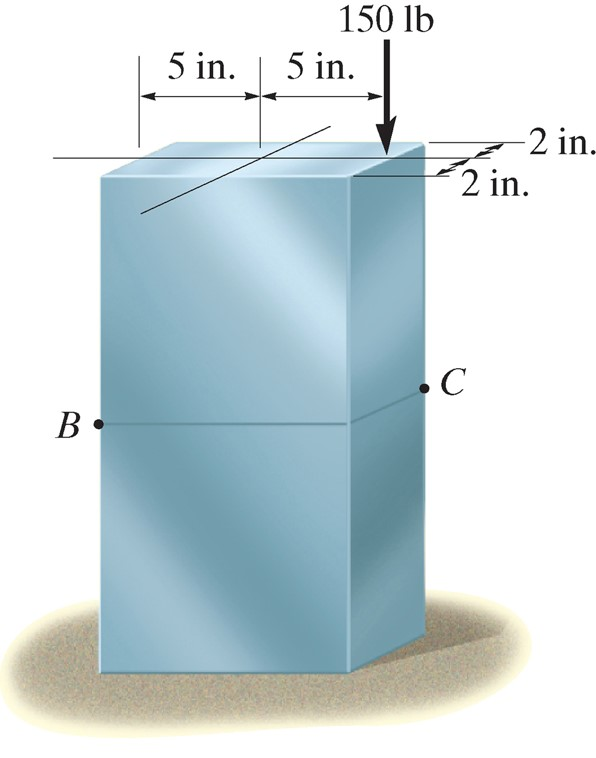
\includegraphics{../images/example-8-2.jpg}

Neglect the weight of the member and find the stress at B and C.
\end{frame}

\begin{frame}{example 8.4}
\protect\hypertarget{example-8.4}{}
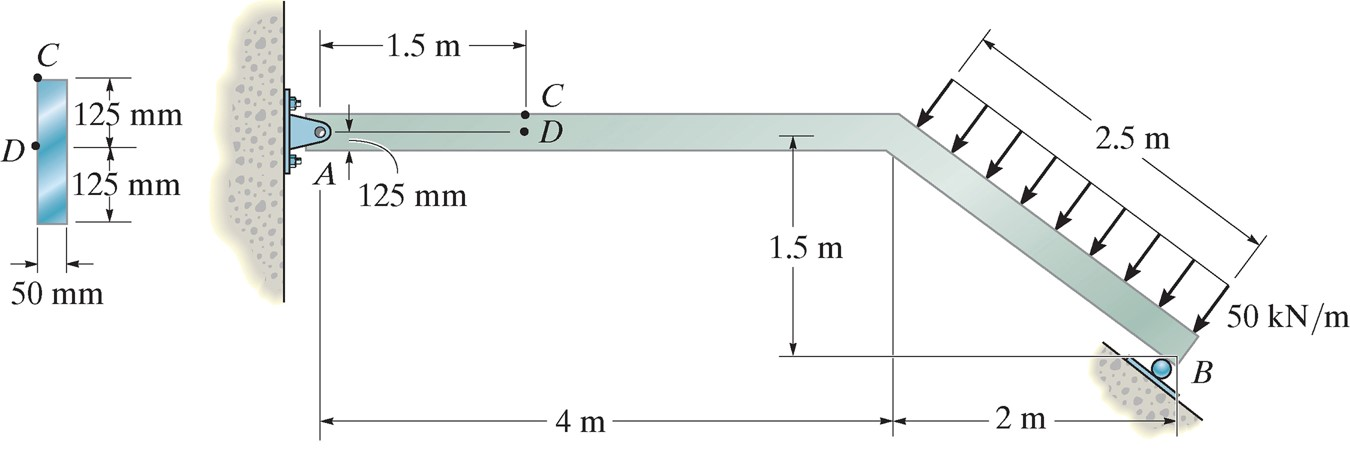
\includegraphics{../images/example-8-4.jpg}

Determine the stress at C and D.
\end{frame}

\begin{frame}{example 8.5}
\protect\hypertarget{example-8.5}{}
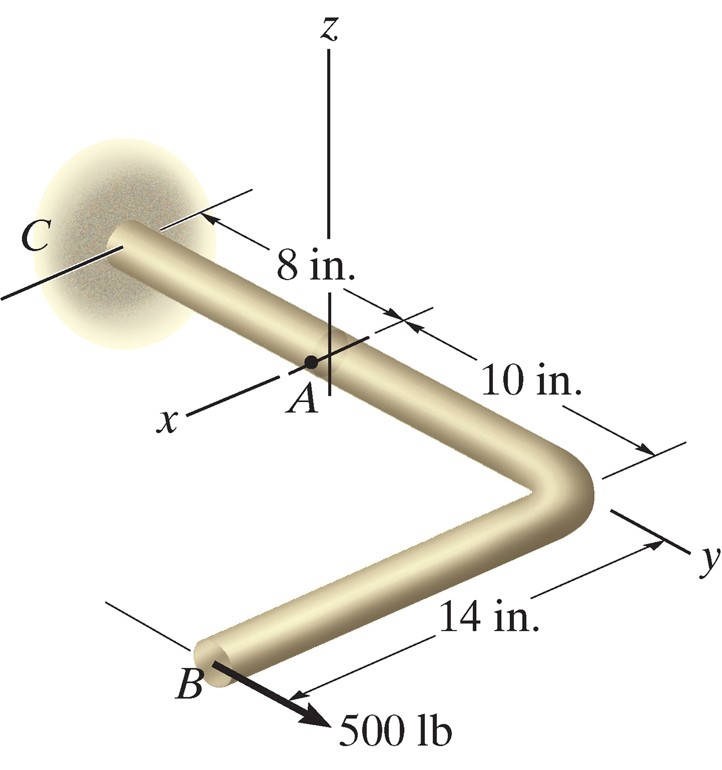
\includegraphics{../images/example-8-5.jpg}

The rod shown has a radius of 0.75 in. Find the stress at A.
\end{frame}

\begin{frame}{group one}
\protect\hypertarget{group-one}{}
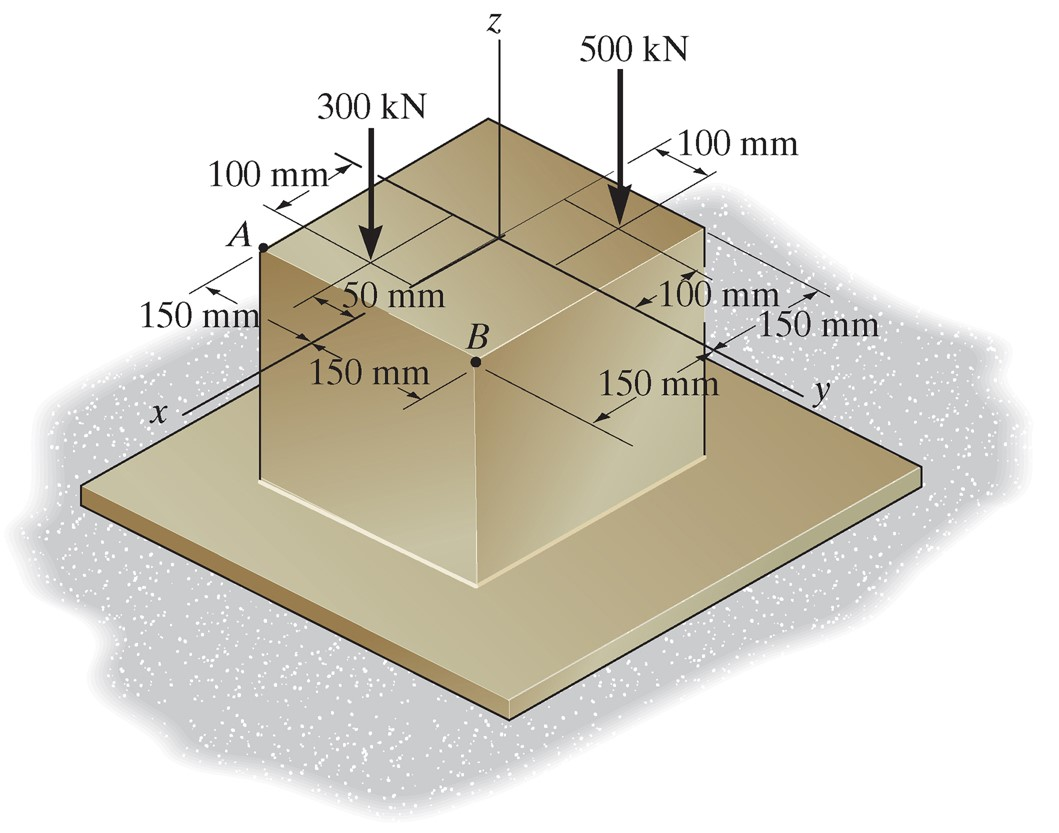
\includegraphics{../images/group-8-1.jpg}

Find the stress at the corners A and B for the column shown.
\end{frame}

\begin{frame}{group two}
\protect\hypertarget{group-two}{}
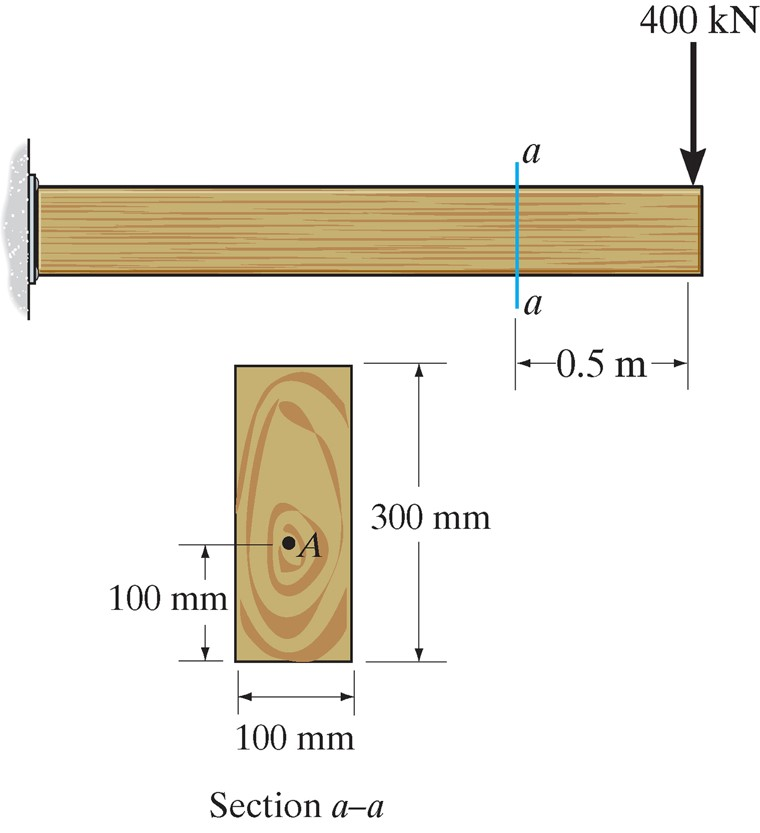
\includegraphics{../images/group-8-2.jpg}

Find the stress at point A for the cantilever beam shown.
\end{frame}

\begin{frame}{group three}
\protect\hypertarget{group-three}{}
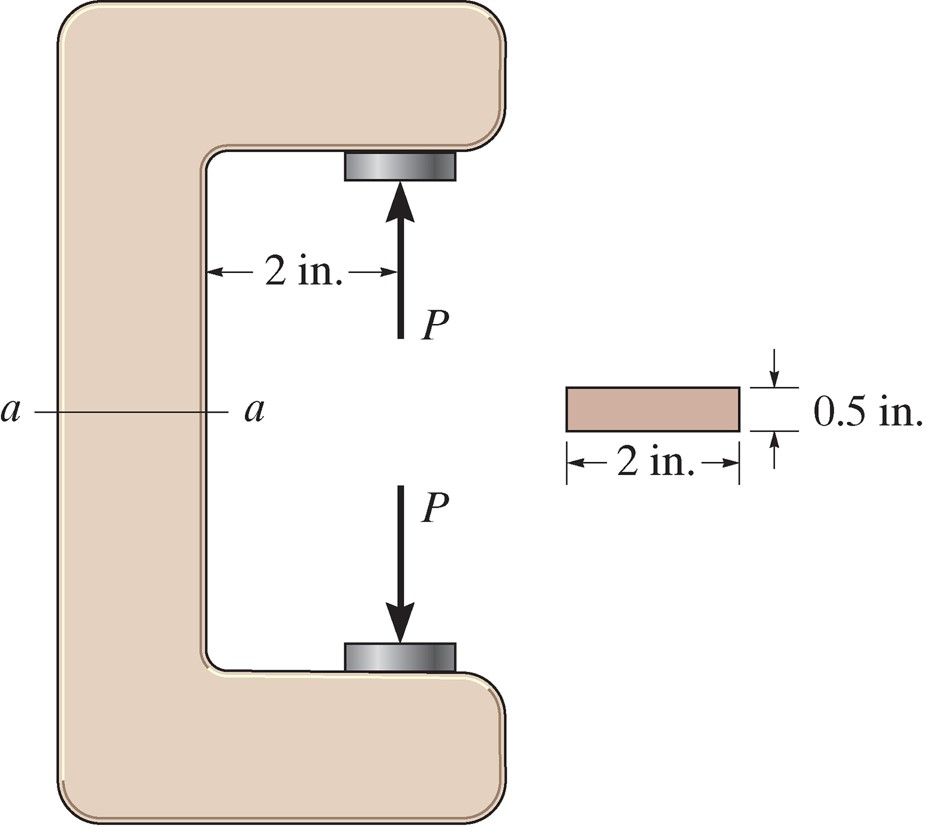
\includegraphics{../images/group-8-3.jpg}

Find the load P that will cause a maximum normal stress of σ=30 ksi
along the section a-a.
\end{frame}

\end{document}
